\section{Contrazioni}
% definizione contrazioni, pag 13.5
\begin{definition}[Contrazione]\label{def:contraz}
    Una contrazione è una funzione $f: \mathbb{N} \rightarrow \mathbb{N}$, per cui vale
    \[ f(n) < n \quad \forall n>n_0 \]
\end{definition}

\subsection{Iterate}
% definizione iterata, pag 13.6
\begin{definition}[Iterata]\label{def:iterata}
    Ad una contrazione sono associate le iterate di $f(n)$
    \[
    \begin{cases} 
        f^{(0)} (n) = n      &  i = 0 \\
        f^{(i)} (n) = f \left( f^{(i-i)} (n) \right)   &  i > 0 \\
        
    \end{cases}
    \]
\end{definition}
Nota: le iterate formano una successione decrescente $ f^{(0)} (n) > f^{(1)} (n) > \cdots > f^{(i)} (n) $ \\
Nella prossima sezione, l'iterata $0$ sarà associata alla radice dell'abero e all'istanza generale, l'iterata $i-esima$ rappresenterà la taglia al livello $i$ dell'albero.

\subsection{Ausiliaria}
% Def ausiliaria, pag 14.6
\begin{definition}[Ausiliaria]\label{def:ausiliaria}
    Alle iterate di una funzione si associa anche una funzione ausiliaria, che indica il maggior indice di iterata per cui il valore è ancora maggiore del valore di base. Nell'albero delle ricorrenze, questo indicherà l'ultimo livello.
    \[ f^*(n, n_0) = \max \{ i>0 : f^{(i)}(n) > n_0 \} \]
    La funzione è definita solo per $n>n_0$, per convenzione assume il valore $f^*(n,n_0)=-1$ se $ n \leq n_0$
\end{definition}

\subsection{Esempi}

\subsubsection{$\bm{f(n) = n/2}$}
% pag 13.9, 14.8
Calcoliamo la forma esplicita dell'iterata e la funzione ausiliaria per
\[ f(n) = \frac{n}{2} \quad \text{con} \quad n=2^k \]
Forma esplicita iterata:
\begin{align*}
    & f^{(0)}(n) = n \\
    & f^{(1)}(n) = f(n) = \frac{n}{2} \\
    & f^{(2)}(n) = f \left( f^{(1)}(n) \right) = f \left( \frac{n}{2} \right) = \frac{n}{4} = \frac{n}{2^2} \\
    & f^{(i)}(n) = \frac{n}{2^i} 
\end{align*}
Dove la generalizzazione  è valida perché gli argomenti restano potenze di due: $n/2^i = 2^{k-i}$ \\
Calcolo funzione ausiliaria:
\begin{align*}
    & f^{(i)}(n) \mgeq n_0 
        & \text{per quali $i\:$?}\\
    & \frac{n}{2^i} \mges n_0 \\
    & 2^i \mles \frac{n}{n_0} \\
    & i < \log_2 \left( \frac{n}{n_0} \right)
        & \text{il vincolo è risolto} \\
    \rightarrow \quad & f^*(n, n_0) = \log_2 \left( \frac{n}{n_0} \right) - 1
        & \text{ne prendo il massimo} \\
    n_0 = 1 \rightarrow \quad & f^*(n, 1) = \log_2 \left( n \right) - 1
        & \text{se $n_0=1$}
\end{align*}

\subsubsection{$\bm{f(n) = n-1}$}
% pag 14, 15
Calcoliamo la forma esplicita dell'iterata e la funzione ausiliaria per
\[ f(n) = n-1 \]
Forma esplicita iterata:
\begin{align*}
    & f^{(0)}(n) = n \\
    & f^{(1)}(n) = f(n) = n-1 \\
    & f^{(2)}(n) = f \left( f^{(1)}(n) \right) = f \left( n-1 \right) = n-1-1 = n-2 \\
    & f^{(i)}(n) = n-i
\end{align*}
Calcolo funzione ausiliaria:
\begin{align*}
    & f^{(i)}(n) \mgeq n_0 
        & \text{per quali $i\:$?}\\
    & n-i \mges n_0 \\
    & i < n - n_0
        & \text{il vincolo è risolto} \\
    \rightarrow \quad & f^*(n, n_0) = n - n_0 - 1
        & \text{ne prendo il massimo} \\
    n_0 = 1 \rightarrow \quad & f^*(n, 1) = n - 2
        & \text{se $n_0=1$}
\end{align*}

\subsubsection{$\bm{f(n) = \sqrt{n}}$}
% pag 14.2, 15.2
Calcoliamo la forma esplicita dell'iterata e la funzione ausiliaria per
\[ f(n) = \sqrt{n} \quad \text{con} \quad n=2^{2^k} \]
Forma esplicita iterata:
\begin{align*}
    & f^{(0)}(n) = n \\
    & f^{(1)}(n) = f(n) = \sqrt{n} = n^{\nicefrac{1}{2}} \\
    & f^{(2)}(n) = f \left( f^{(1)}(n) \right) = f \left( n^{\nicefrac{1}{2}} \right) = n^{\nicefrac{1}{2^2}} \\
    & f^{(i)}(n) = n^{\nicefrac{1}{2^i}} \\
\end{align*}
Calcolo funzione ausiliaria:
\begin{align*}
    & f^{(i)}(n) \mgeq n_0 
        & \text{per quali $i\:$?}\\
    & n^{\nicefrac{1}{2^i}} \mges n_0 \\
    & \log_2 n^{\nicefrac{1}{2^i}} \mges \log_2 n_0 \\
    & \frac{1}{2^i} \log_2 n \mges \log_2 n_0 \\
    & 2^i \mles \frac{\log_2 n}{\log_2 n_0} \\
    & i < \log_2 \frac{\log_2 n}{\log_2 n_0} 
        & \text{il vincolo è risolto} \\
    & i < \log_2 \log_2 n + \log_2 \log_2 n_0 \\
    \rightarrow \quad & f^*(n, n_0) = \log_2 \log_2 n + \log_2 \log_2 n_0 - 1
        & \text{ne prendo il massimo} \\
    n_0 = 2 \rightarrow \quad & f^*(n, 2) = \log_2 \log_2 n - 1
        & \text{se $n_0=2$}
\end{align*}
Il vincolo su $n$ può essere generalizzato a $n=a^{2^k}$, in questo caso $n_0 = a$

\subsubsection{$\bm{f(n) = \left\lfloor n/2 \right\rfloor}$}
Nel caso $f(n) = \left\lfloor n/2 \right\rfloor$, si può dimostrare che
$ f^{(2)}(n) = \left\lfloor \left\lfloor n/2 \right\rfloor / 2 \right\rfloor = \left\lfloor n / 2^2 \right\rfloor $
ma non è per niente banale.

\section
[Modifica al \textit{Divide and Conquer}]
{Modifica al \textit{Divide and Conquer} \\ 
{ \large Risoluzione di una classe generale di ricorrenze\\ associate ad algoritmi \textit{Divide and Conquer} } }
% titolo meno informativo della storia
% sottotitolo già meglio
\subsection{Meta-algoritmo}
% Metaalgoritmo DnC modificato, pag 12.5
\begin{algorithm}[H]
\caption{Divide and Conquer modificato}\label{alg:dncm}
\begin{algorithmic}[1]
    \Procedure{D\&C}{$i$}
        \State $n=|i|$
        \If{$n \leq n_0$}                             \Comment{BASE}
            \State *risolvo direttamente*
        \EndIf
        \State $<i_1, i_2, \dots, i_{S(n)}> \gets A_D(i)$    \Comment{DIVIDE}
        \For{$j \gets 1 $ to $ {S(n)} $ }                    \Comment{RECURSE}
            \State $s_j \gets $ \Call{D\&C}{$i_j$}
        \EndFor
        \State $s \gets A_C(<s_1, s_2, \dots, s_{S(n)}>)$    \Comment{CONQUER}
        \State return $s$
    \EndProcedure
\end{algorithmic}
\end{algorithm}
% Parametri noti, pag 13
L'algoritmo ha dei vincoli in più rispetto al prototipo generico, in particolare sul numero e dimensione delle sottoistanze generate. I parametri che lo descrivono sono:
\begin{itemize}[noitemsep,topsep=0pt,parsep=0pt,partopsep=0pt]
    \item[--] $S(n): \mathbb{N} \rightarrow \mathbb{N}$ \\
        istanze di taglia $n$ nella fase di \textit{Divide} generano sempre lo \textbf{stesso} numero di sottoistanze
    \item[--] $ |i_j| = f(n) < n \quad \forall j : 1 \leq j \leq S(n) $ \\
        le sottoistanze sono sempre grandi uguali
    \item[--] $ w(n) = T_{A_D}(n) + T_{A_C}(n)$ \\
        lavoro compiuto per ogni istanza per dividere e ricomporre
    \item[--] $n_0$ taglia del caso base
    \item[--] $T_0$ tempo al caso peggiore di risoluzione diretta quando $|i| \leq n_0$
\end{itemize}
% Nuova eq di ricorrenza, pag 13.3
L'equazione di ricorrenza diventa
\[
    T(n) = 
    \begin{cases} 
        T_0      &  n \leq n_0 \\
        S(n) \, T(f(n)) + w(n) & n > n_0
    \end{cases}
\]
Ad ogni passo vengono fatte $S(n)$ chiamate ricorsive su istanze grandi $f(n)$

\subsubsection{esempio parametri MAX}
% parametri max, pag 13.5
I parametri del $MAX$ sono, con la nuova notazione:\\
$S(n)=2$, $f(n)=n/2$, $w(n)=1$, $T_0=0$, $n_0=1$

\subsection{Equazione delle ricorrenze generica}
% Alberone, pag 15.8
{ \centering
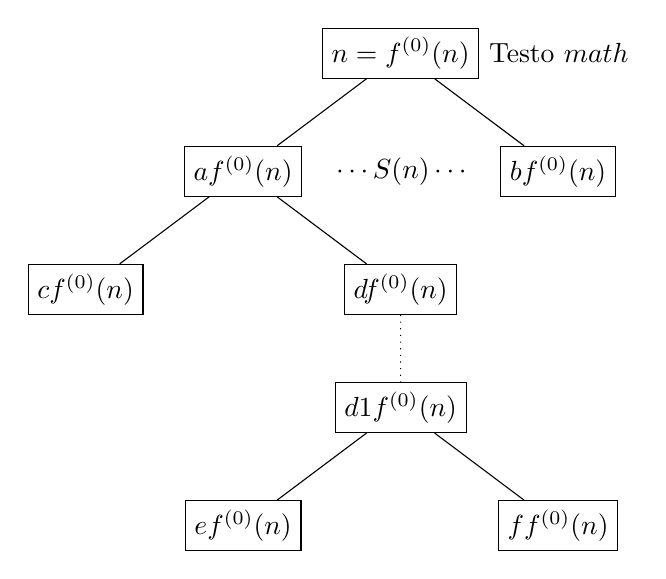
\begin{tikzpicture}[
    level/.style={sibling distance=40mm},
    every node/.style={rectangle,draw,solid},
    dotme/.style={edge from parent/.style={dotted,draw}},
    norm/.style={edge from parent/.style={solid,draw}}
    ]
    \node [label=right:{Testo $math$}] (z){$n = f^{(0)}(n)$}
        child { node (a) {$a f^{(0)}(n)$}
            child { node  (c) {$c f^{(0)}(n)$}
            }
            child { node  (d) {$d f^{(0)}(n)$}
                child [dotme] { node (d1) {$d1 f^{(0)}(n)$}
                    child [norm] { node  (e) {$e f^{(0)}(n)$}
                    }
                    child [norm] { node  (f) {$f f^{(0)}(n)$}
                    }
                }
            }
        }
        child { node  (b) {$b f^{(0)}(n)$}
        }
    ; % end of the node
\path (a) -- (b) node [draw=none,midway] {$\cdots S(n) \cdots$ };
\end{tikzpicture}

} % end centering, LASCIA la riga sopra questa parentesi (serve un \par)
% Formulone, pag 16
\begin{align*}
    T(n) & = \sum_{l=0}^{f^*(n,n_0)}\text{\# nodi nel livello}\cdot\text{\# $w$ per nodo del livello}+\text{contributo foglie}\\
    &= \sum_{l=0}^{f^*(n,n_0)} \left[ \prod_{j=0}^{l-1} S \left( f^{(j)}(n) \right) \cdot w \left( f^{(l)}(n) \right) \right] +
        \prod_{j=0}^{f^*(n,n_0)} S \left( f^{(j)}(n) \right) \cdot T_0
\end{align*}

Da qualche parte le convenzioni sugli operatori, pag 15.5; insieme alle cose a fine capitolo DnC -> Appendice

\subsubsection{Esempio formula}
Esempio, pag 16.5

\subsubsection{Esempio formula}
Esempio, pag 17.5

\section{\textit{Master theorem}}
Ipotesi, pag 18

Tesi, pag 18.5

Dimostrazione, pag 20

Considerazioni sull'asintotico, pag 18.9, 19

\subsection{autocomplete}
Una bella scatola:
\begin{equation}
    \boxed{x^2+y^2 = z^2}
\end{equation}

àg
èg
ìg
òg
ùg
perché

